\section{Triggers}
    In the triggers section you can define which triggers to apply for a given probe, once selected, they will be automatically activated.

    Once a trigger is triggered, the oscilloscope will keep recording the system for a few seconds. Once stopped, under the "snapshots" section, you can click the snapshots to view them in a separate section, there, you can observe the $\Delta$Qs of all the probes before and after the trigger was triggered. You can discard the snapshot by left clicking on it and clicking \textit{"Delete snapshot"}.

     \begin{figure}[H]
        \begin{center}
        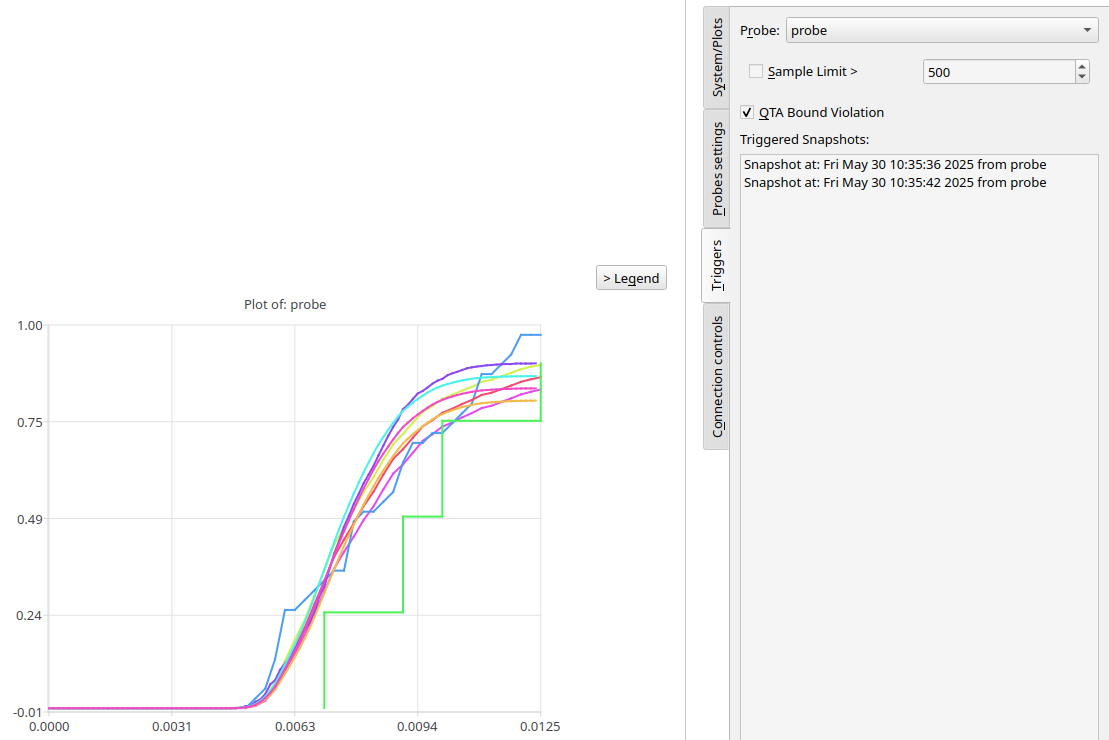
\includegraphics[width = \textwidth]{img/manual/triggers.png}
        \end{center}
        \caption{Examples of the QTA being set for a probe "probe". Once a trigger is fired, the resulting snapshot from the fired trigger will be available under "Triggered snapshots".}
    \end{figure}

\section{Snapshots}
    The snapshots can be observed to look at the state of the system, before, during and after the trigger has been fired.

    By clicking on the snapshot in the "triggered snapshots" section, a new window will popup where you can observe the system. A slider allows you to move backwards and forwards in time, observing the state of a probe in time.
 
    \begin{figure}[H]
        \begin{center}
        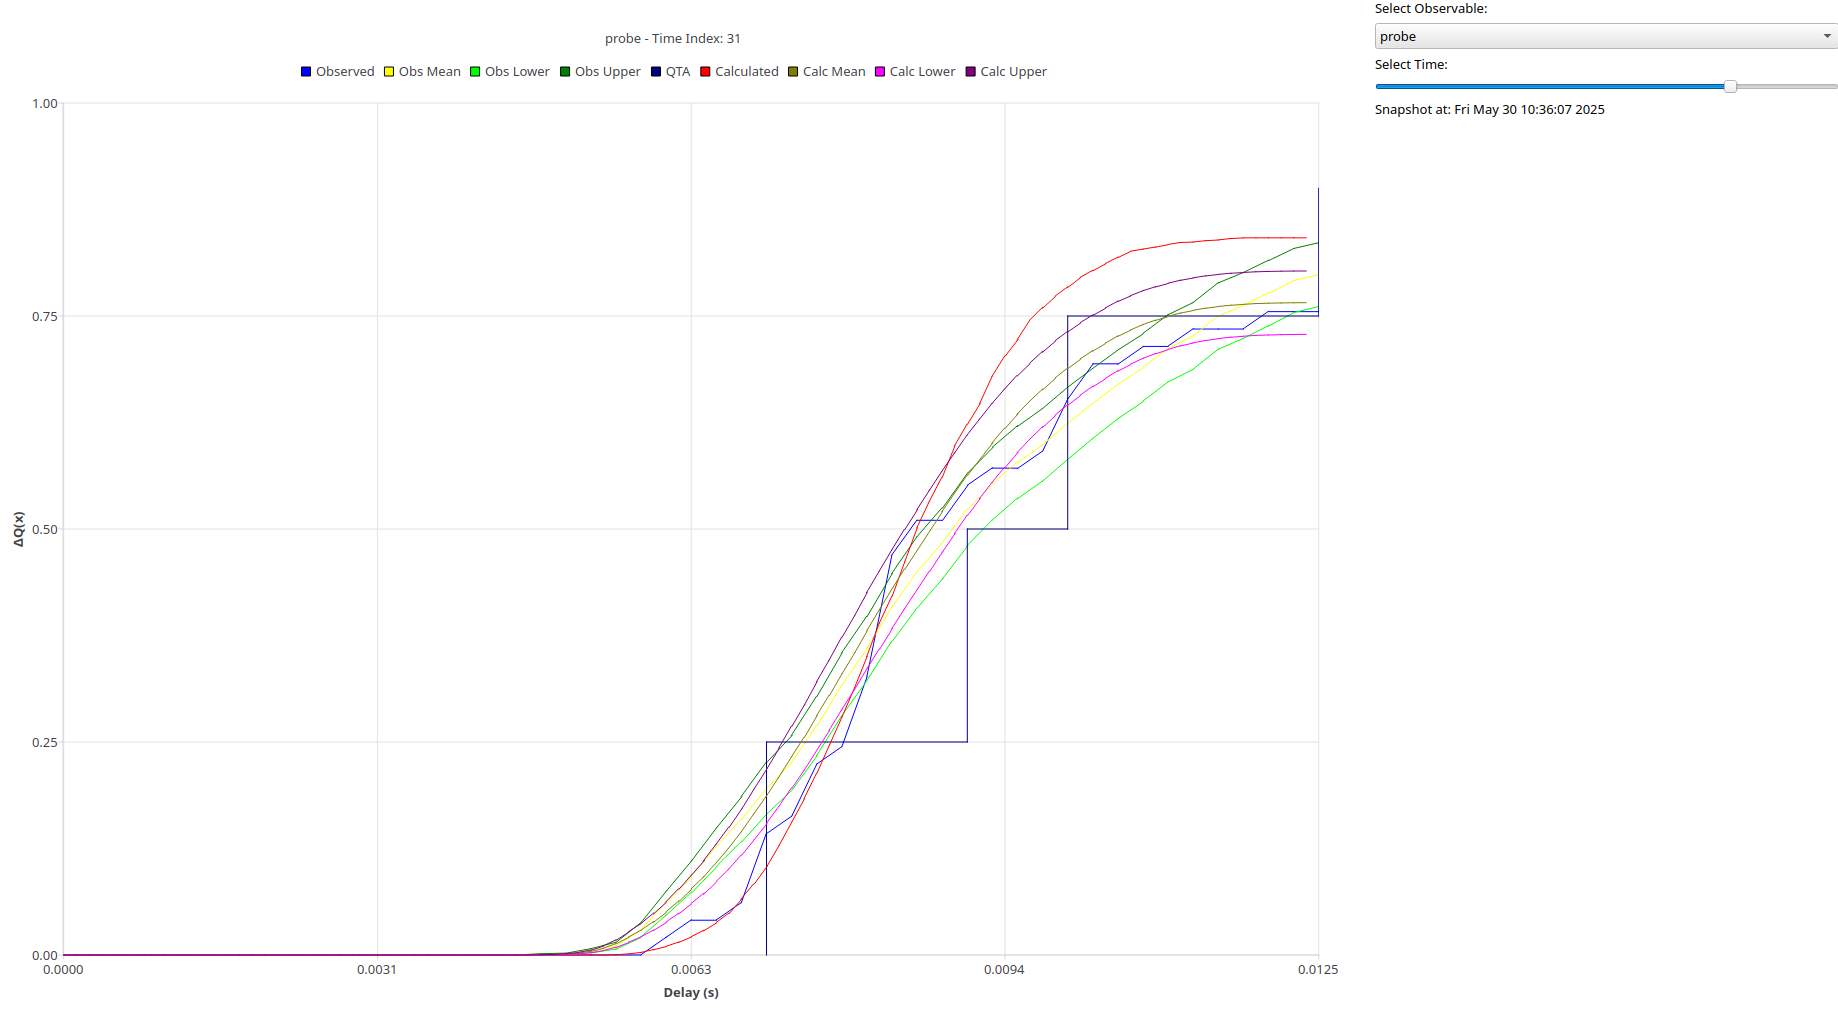
\includegraphics[width = \textwidth]{img/manual/snapshot.png}
        \end{center}
        \caption{Example of a snapshot, to the left, the graph at time $t$. To the right, the time of the graph on the left and a slider to advance backwards and forwards. As of right now, you can only select a probe at a time.}
    \end{figure}
